\section{Voorraadbeheer}

\subsection{Inleidende Beschouwingen}
Bij het beheer van de voorraad wil je er voor zorgen dat er niet te veel en niet te weinig is. Optimalisatie van de voorraad is een zeer belangrijk onderdeel in heel wat bedrijven.

Voorraad = goederen/producten die je aanhoudt voor toekomstig gebruik. Ze ziojn dus nuttig, maar ze vertegenwoordigen dus ook een ge\"investeerd kapitaal dat vast staat. Bijgevolg is voorraad vaak van strategisch belang voor bedrijven.

Toenemende productvari\"eteit (groter aantal SKU's) zorgt dat voorraden ook niet zo sterk dalen ondanks de constante druk om de voorraden te doen afnemen.

\subsection{Definitie}
Een voorraad zijn dus goederen die je aanhoudt voor toekomstig gebruik. In principe zijn er vier verschillende soorten voorraden:
\begin{itemize}
    \item Hulpstoffen
    \item Grondstoffen
    \item Goederen in bewerking (work in progress)
    \item Afgewerkte producten
\end{itemize}

\subsection{Belang van voorraadvorming}
Voorraden worden aangehouden omdat het fysisch onmogelijk is, of economisch onverantwoord is of te risicovol is om goederen te laten toekomen juist op het moment dat er een vraag naar is (\textit{op voorraad produceren}). Zonder voorraad moet de klant wachten (\textit{op order produceren}).

\begin{figure}[htbp]
    \centering
    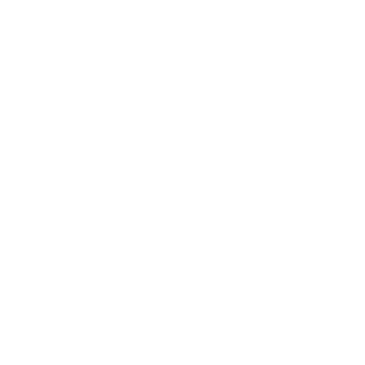
\includegraphics[scale=0.4]{Images/white.png}
    \caption{De totale logistieke keten (fig 1 boek)}
    \label{fig:totaleLogistiekeKeten}
\end{figure}
Als we naar de totale logistieke keten (figuur~\ref{fig:totaleLogistiekeKeten}) kijken zien we dat voorraden zich op meerdere plaatsen zullen vormen. Er zijn drie voorname redenen voor dit fenomeen:
\begin{description}
    \item[Tijd- en ritmeverschillen (fysisch)] Levertijden en productieduur zorgen dat er voorraad aangehouden moet worden als buffer om deze duurtijden te kunnen overbruggen. De voorraad kan gedrukt worden door productie op vraag af te stemmen en het inkorten van de totale doorlooptijd. Bij dit aspect spelen dus voornamelijk de overgangen tussen de verschillende spelers in de logistieke keten.
    \item[Onzekerheid en variabiliteit (risico)] Leveringstermijnen kunnnen veranderen, vraag is onzeker, machines kunnen uitvallen, \dots Deze onzekerheid geeft aanleiding tot het aanhouden van voorraad. Het wegnemen van deze onzekerheden laat toe de voorraad te verkleinen. Als je aan dit aspect denkt wil je dus voornamelijk vermijden op order te produceren.
    \item[Economisch motief (economisch)] De grootte van de voorraad hangt af van een \textit{trade-off analyse}, zoals we later zullen zien, om de kosten te minimaliseren. Voorraad ontstaat dus ook dankzij dit motief.
\end{description}

\subsection{Componenten van een Voorraadsysteem}
De belangrijkste componenten zijn: de \textit{vraagstructuur}, de \textit{aanbodstructuur}, \textit{beperkingen} en \textit{kosten} en tot slot \textit{service}.

Bij de vraag maken we een eerste onderscheid tussen \textit{onafhankelijke/afhankelijke} vraag, waarbij onafhankelijk de marktvraag van het eindproduct is (meestal niet gekend), de afhankelijke vraag de vraag naar componenten is. Daarnaast kan de vraag ook constant/variabel en gekend of ongekend zijn (stochastisch vs. deterministisch model).

Op vlak van de aanbodstructuur denken we aan de aankoop of productiemodellen van het bedrijf zelf. Bij productiemodellen spelen \textit{omsteltijden}, \textit{productiesnelheid} en \textit{wachttijden} voor machines mee.

Beperkingen kunnen van allerlei aard zijn.

De kosten die meespelen zijn de volgende:
\begin{description}
    \item[Bestel- of omstelkosten] Deze kosten gaan gepaard met het plaatsen van een bestelling of het opstarten van productie waarbij machines omgesteld moeten worden. In het algemeen kunnen deze kosten opgedeeld worden in \textit{transportkosten} en \textit{handling-in- en out-kosten}.
    \item[Aankoopprijs] Uiteraard heeft de prijs van een product een impact op de aankoopkosten ervan. Indien men zelf produceert rekent men als aankoopkost de prijs van de grondstoffen plus directe kosten zoals arbeid en een toeslag voor indirecte kosten.
    \item[Voorraadkosten] Een voorraad aanhouden kost geld, en dit vanwege een paar redenen. Eerst is er de \textit{kapitaalkost}. Geld dat vastzit in de voorraad had men voor andere doeleinden kunnen gebruiken. Daarnaast moet men ook betalen voor de \textit{opslagruimte} en de \textit{behandeling} van de voorraad. Tot slot speelt \textit{veroudering} van de voorraad mee waardoor deze op termijn waarde kan verliezen.
    \item[Tekortkosten] Tekortkosten zijn iets anders dan de voorgaande kosten. Het gaat hier om \textit{gederfde winst}. Indien het goed in voorraad had geweest, had men dit kunnen verkopen en hier winst op kunnen maken. Nu is dit niet het geval en bestaat de kans dat deze potenti\"ele klant naar de concurrentie gaat.
\end{description}

Tot slot is er nog de \textit{service}. Men zal vaak een zo goed mogelijke service aan de klant nastreven (=het gewenste goed meteen kunnen leveren). Bijgevolg zal men voorraad moeten aanhouden.

Een voorraadmodel kunnen we uitdrukken aan de hand van een \textbf{doelfunctie} die we gebruiken om de kosten te minimaliseren, terwijl we voldoen aan een bepaald \textit{serviceniveau}.


\subsection{Het Meten van Voorraad}
Een eerste methode om de voorraad te meten zijn de zogenamde \textbf{statische maatstaven}. Het gaat hierbij om de klassieke balans-ratio's, de voorraadwaarde, $\frac{\text{voorraadwaarde}}{\text{omzet aan kostprijs}}$ en de voorraadrotatie.

De \textbf{dynamische maatstaven} gaan de voorraad doorheen de tijd beschrijven/analyseren. We zien twee voorbeelden:
\begin{description}
    \item[Voorraadprofiel]: het voorraadprofiel geeft weer wat de waarde van de voorraad in functie van de tijd is (zie fig 2 boek). In het begin is dit alleen de waarde van de grondstoffen, maar hier komen uiteindelijk nog verwerkingskosten etc. bij. Indien we weten wat de waarde van de totale jaarproductie is, kunnen we de oppervlakte onder de curve van het voorraadprofiel berekenen. Wanneer we de totale jaarproductie door dit getal delen kennen we de voorraadrotatie.

    \item[(Cumulatieve) Input-outputgrafiek] Met deze voorstellingsmethode wil men alle schakels in een productiesysteem weergeven (zie fig 3\&4 boek). Denk hierbij aan een aantal trechters die in elkaar over gaan. Een andere voorstelling is de cumulatieve I/O grafiek in functie van de tijd (fig 5 boek), waarin een horizontale doorsnede tussen input en output de doorlooptijd weergeeft en verticale de voorraad op een bepaald tijdstip.
\end{description}

Vervolgens introduceren we de \textbf{wet van Little}. Deze wet stelt dat:
\begin{equation}
    \boxed{\text{gemiddelde voorraad} = \text{gemiddelde doorlooptijd} \times \text{gemiddelde input}}
\end{equation}
en toont duidelijk het verband tussen doorlooptijd en voorraad. Als we er van uitgaan dat gemiddelde input gelijk is aan gemiddelde output (wat binnen komt gaat ook terug weg), kunnen we dat verband ook met gemiddelde productie leggen.
